\documentclass{article}

% Include AMS packages
\usepackage{amsmath,amsthm,amssymb}
\usepackage{tikz}
\usepackage{listings}
\usepackage{pgfplots}
\usepackage{graphicx}
\usepackage{enumitem}
\usepackage{xurl}
\usepackage{parskip}
\usepackage{placeins}
\usepackage{float}

\usetikzlibrary{automata,topaths}

\graphicspath{{C:/Users/sjdmu/Documents/GroupProject}}

\lstset{breaklines=true, language=Python, basicstyle=\footnotesize, showstringspaces=false}

\pgfplotsset{compat=1.16}

\author{Sebastian Murden, Zachary Dawkins, \\ Thomas Hanstock, Megan Potter}

\date{}

\begin{document}




\title{Modelling the Role of Disease in the Decline of Red Squirrels}
\maketitle

\tableofcontents

\section{Introduction}

Red squirrels are a species which is native to the UK, but their population has taken a considerable decline over the past few decades and are now only found in specific areas of Wales, Scotland and England as seen in figure 1. [8] At first, this was largely thought to be due to competition from the imported North American grey squirrel. However, the decline in the numbers of red squirrels was way too severe to be down to competition alone. The findings in recent years suggest that the parapox virus, a disease where grey squirrels are immune but is fatal to red squirrels, has played a large role in the decline of the red squirrels across the UK.

\begin{figure}[H]
\begin{center}
\includegraphics[width=0.7\textwidth]{ukmap}
\caption{A distribution map comparing red and grey squirrels in 1945 and 2016 [13].}
\end{center}
\end{figure}

In this project, we will use mathematical modelling of ordinary differential equations to look at both competition and disease further and analyse whether the presence of disease does indeed speed up the rate of decline in red squirrels.  We will also look into a small grid model to demonstrate the replacement of red squirrels with grey squirrels will behave over a small grid.




\section{Biological Background}

The Eurasian red squirrel, or \emph{Sciurus Vulgaris} in Latin [1], is the only native squirrel species in the British Isles.  Red squirrels colonised the British Isles around 10,000 years ago during the last ice age [9]. Around this time, the red squirrel would have been present in large quantities across suitable forests across the UK, as seen in Figure 1 [9]. However, red squirrel numbers are significantly declining and are now only present in very few forests across the UK [2]. Due to the rapidly declining numbers, the UK government has made it a priority to protect the remaining red squirrel populations [10].

\begin{figure}[H]
\begin{center}
\includegraphics[width=0.7\textwidth]{squirrelpic}
\caption{Annotated image size of Red and Grey Squirrels [14].}
\end{center}
\end{figure}

Between 1400-1600, there was a dramatic reduction of the number of red squirrels in the UK due to deforestation because of agriculture. This continued through until the mid-1800’s and red squirrel numbers continued to decline due to deforestation, where the numbers got so low the squirrels got close to extinction in Scotland. However, from 1875-1910, the numbers began to increase due to tree and woodland planting, giving squirrels the perfect habitat to live in. In fact, the numbers got so high again that they were considered ‘pests’ in the early 1900’s, which led to ‘squirrel clubs’ beginning to hunt the species. As well as the hunting, squirrel numbers again started to decline in 1914 due to loss of forests and woodland as part of material collecting for World War 1. [9]

It is clear to see that red squirrel numbers have both decreased and increased overtime due to woodland habitat, however with the second world war being over, woodland planting started again. It was expected that the red squirrel numbers would again start to rise as it had when the first world war was over, but this wasn’t the case. [9]

An introduction of the North American Eastern grey squirrel, or \emph{sciurus carolinensis}, [1] in the late 1800’s and early 1900’s to the UK wild meant the red squirrels had another competitor. This new competitor is known to strip bark off of trees causing tree death which leads to loss in woodland resources [9], a known cause for red squirrel population decline. Grey squirrels increased in large numbers throughout the 20th century, and were even considered a ‘pest’ in the 1930’s. In the 1970’s, it was considered that the dramatic increase of the number of grey squirrels coincided with the reduction of the number of red squirrels [9].

Having realised the change in numbers of both species were related, scientists began to wonder why this was happening. There was no evidence of aggressive behaviour between the two species, the two species are generally very tolerant of each other when the two species share a habitat [9].



There is evidence to show that grey squirrels do steal red squirrels’ food, grey squirrels are bigger than red squirrels, as seen in Figure 2, and so they have been known to outcompete the red squirrels for food and territory. This means that female red squirrels produce fewer young per litter as well as often only producing one litter per year instead of the potential two litters per year. This would lead to a slight decrease in the number of red squirrels. [9][10]

From this it’s clear that the introduction of grey squirrels has had an impact on the number of red squirrels. However, the amount that the red squirrels population was declining couldn't have been just down to competition alone, another factor must have been playing a part. 

Scientists would then go on to realise that grey squirrels carried a virus with them called Squirrel Pox Virus (SQPV) which is fatal to red squirrels while grey squirrels are immune, it was suggested that this could be a key reason behind the decline of the red squirrel population. [9]




\section{A Simple Model}

To demonstrate the impact of introducing a grey squirrel to the red squirrel population, we focused on one red squirrel and produced a model that illustrated the effect on this red squirrel’s life and therefore the effect on the population after this interaction.

\begin{figure}[H]
\begin{center}
\includegraphics[width=0.9\textwidth]{flowchart}
\caption{Flow chart for simplified model (made on lucid chart by us).}
\end{center}
\end{figure}

Figure 3 introduces one grey squirrel to one red squirrel and investigates all of the factors of a squirrel’s life that we found earlier have been affected by the grey squirrel introduction. If we investigate a short term study of one year, the simplicity of the model means that there are 3 possible outcomes of the model;

\begin{enumerate}
\item An increase in population by a litter size shown in Figure 3 by the green outcome which we refer to as outcome 1, 
\item A constant population shown in Figure 3 as a yellow outcome which we refer to as outcome 2, 
\item A decrease in the population by one shown in Figure 3 by a red outcome which we refer to as outcome 3. For simplicity, this model does not include a smaller litter size for now.
\end{enumerate}

So in terms of population, the changes are as follows:

\begin{equation}
  \Delta R = R_{t+1} - R_{t} =
    \begin{cases}
      +x & \text{if outcome 1}\\
      0 & \text{if outcome 2}\\
      -1 & \text{if outcome 3}
    \end{cases}       
\end{equation}

In Equation 1, we have defined the changes in the population per unit time which here we defined as the breeding season and we get 3 possible outcomes to the population. Outcome 1 being when the red squirrel has ideal condition and resources to breed, with $x$ being the litter size. Outcome 2 being the constant population where the red squirrel survives but does not breed because of possibly a lack of breeding grounds. Outcome 3 being the situations where the red squirrel dies either due to the strain on the resources brought about by the introduction of the grey squirrel, or by contracting squirrel pox from the grey squirrel carrier. 

After the second world war, when the start of red squirrel population decline began, it was thought that red squirrel numbers should be rising as seen after the first world war. If we considered a scenario where the grey squirrels were not introduced, we could assume that a single red squirrel had two breeding seasons, due to plentiful resources, and we can assume that Natural mortality rates for red squirrels were also low. Due to this, we get an expected population change in this system: 

\begin{equation}
  \Delta R = R_{t+1} - R_{t} =
    \begin{cases}
      +2x & \text{if outcome 1}\\
      0 & \text{if outcome 2}\\
      -1 & \text{if outcome 3}
    \end{cases}       
\end{equation}


In equation 2, it is important to note that we have not taken into account the possible increase in litter size of the red squirrels for the simplicity of our initial model. Not only this, the probabilities of outcome 2 and 3 occurring are much lower in this model as resources are much more plentiful so death from lack of resources and not breeding from lack of resources is much less likely. From this it is clear to see the impact of the grey squirrel invasion.

This model is very simplistic, however it does give us a good idea and understanding for how to further develop our study of the population. This model shows that with just including one squirrel, the difference in possible population sizes for after the breeding season is $x+1$ which shows that in a population of 120,000 red squirrels [6], this has a large variation in population and with using the idea of likelihood mention above we can conclude that though the model shows a limited effect that in fact the effect of the grey squirrel introduction could have a maximum possible population decrease: 

\begin{equation}
\Delta R = R_{t+1}-R_{t}=P_{R}-P_{R}'(x+1).
\end{equation}

In Equation 3, we define $P_{R}$ to be the population size of red squirrels at the beginning of the study and $P_{R}'$ being the population of red squirrels who are capable of producing a litter and $x+1$ being the maximum decrease in population size for each red squirrel. 

This was interesting because when investigating this simple model we found that the system demonstrated that the grey squirrels clearly had an impact on the population size of the red squirrels. This model is not suitable though because it does not account for the possible death of both parents to the litter in question. This problem could be easily solved by changing the initial model from one adult to two adults, then the maximum deaths in this system would be $x+2$ instead. This system still is not preferable because there is a high likelihood that the male would have fathered more than one litter each breeding season, so it is ineffective to pair off the squirrels in this manner. Not only this, but we also do not take into account here the transmission of squirrel pox or the fecundity.








\section{Population Growth Modelling}

We will now look at some simple ways of modelling population, these include Basic, Exponential and Logistic growth models. Using these, we can observe how the population of species, in particular red squirrels, can grow and look at ideal conditions for red squirrels to thrive. However, populations not only grow, but also deplete. As previously mentioned, red squirrel numbers have both increased and decreased overtime due to a number of factors, which we will later look at in more detail. For now, we shall look at the mathematics of population growth.

The population of any species within an environment of unlimited resources grows exponentially, regardless of population size, making the population grow at an increasing rate as it gets larger. Theoretically, any species could take over the whole world with just reproducing and when encountering zero resistance to its growth. Realistically however, there are a multitude of factors inhibiting this from happening such as availability of food and water, space, predation, disease, shelter, competition for resources and many more. With the Earth’s limited resources, exponential growth cannot continue indefinitely - as population size increases, resources will be depleted, slowing the growth rate, and which will eventually cause it to plateau. Thus the population will come to its equilibrium at a natural, maximum population size that the environment can support sustainably and this quantity is called the \textbf{carrying capacity}. This term is like a natural “ceiling” for population dynamics. Once the population size surpasses the carrying capacity, the limitations on resources as well as other factors cause an increase in the mortality rate to a point that it outweighs the natality rate, this brings the population back down to its carrying capacity. 

Over the years, scientists have modelled populations and their growths using various models and techniques which each use numerous factors and parameters affecting the results. A simple example of a population model is the equation:

\begin{equation}
\frac{dN}{dT}=rN.
\end{equation}

Here in Equation 4, we have $\frac{dN}{dT}$ denoting the rate of change in population size at each time point $T$, and $r$ and $N$ are the rate of reproduction and population size respectively. This demonstrates that the growth rate is equal to the population size multiplied by some factor.  This is the most basic and general model for population dynamics, so whilst this acts as a good model to predict how red squirrel population dynamics may change, we need to adapt these to become more detailed and specific models to become more naturalistic and representational of the real world. So, we will now look at an exponential model.


\subsection{\textbf{Exponential Growth}}

Here we consider an advancement forward from our basic equation to exponential growth within an ideal world and the key concept of exponential growth is that the population growth rate increases as the population gets larger. Any positive, constant value of $r$ in the above equation can lead to exponential growth. Using a graph of population against time, we can see a J-shaped curve is formed when observing exponential growth. [4]

\begin{figure}[H]
\begin{center}
\begin{tikzpicture}
\begin{axis}[xlabel=Time, ylabel=Population size,  yticklabels={0}, xticklabels={0}, axis x line=middle,
    axis y line=middle, extra x ticks = {0}]
\addplot[color=red, domain=0:5]{exp(x)};
\end{axis}
\end{tikzpicture}
\caption{Exponential growth graph.}
\end{center}
\end{figure}

This is written as:
$$\frac{dN}{dT}= r_{max}N.$$
and we have written $r_{max}$ since this is the maximum per capita rate of increase for a particular species under ideal conditions.[11]


\subsection{\textbf{Logistic Growth}}

The exponential growth population model is the basis for the logistic growth model but now $r$ will be decreasing as the population increases towards its limit. There will be a phase of exponential growth occurring for a short while when there are surplus resources available for the current population, however due to reality and limited resources it will plateau. This is due to reasons we stated before and can be plotted to show an S-shaped curve where the carrying capacity $K$ comes into play.

\begin{figure}[H]
\begin{center}
\begin{tikzpicture}
    \begin{axis}%
    [     
        xlabel=Time,
        ylabel=Population size,
        xmin=-6,
        xmax=6,
        axis x line=bottom,
        xtick={\empty},
        ymax=1.5,
        axis y line=left,
        yticklabels={0}, xticklabels={0},
        ytick={1.03},
        yticklabel={$K$}
    ]
        \addplot%
        [
            blue,%
            mark=none,
            samples=100,
            domain=-6:6,
        ]
        (x,{1/(1+exp(-x))});
            \end{axis}
\draw[red, thick, dashed](0,3.9)--(6,3.9);
\end{tikzpicture}
\caption{A graph showing logistic growth.}
\end{center}
\end{figure}

We model this by slightly adjusting our equation for exponential growth. Again, $r$ is growth rate and $N$ is population size, however, we now add the carrying capacity $K$ into this model since the population now depends on how close it is to the carrying capacity. We write the following equation:

$$\frac{dN}{dT}=rN\frac{K-N}{K}.$$

Now, let's see how this equation makes sense. Looking at the fraction of $\frac{K-N}{K}$ [4] we can see that when $N$  is very small, the fraction becomes almost $\frac{K}{K}$, or 1, and this just gives us the exponential growth that we had previously. When $N$ grows and approaches $K$, the fraction becomes very small and this levels off the growth rate.

The key point of the logistic population growth model is that it occurs when a population's \emph{per capita} growth rate decreases as the population size approaches the carrying capacity $K$.




\subsection{\textbf{Lotka-Volterra Model}}

In the late 1920s, two researchers, Alfred J. Lotka and Vito Volterra, independently derived a way to use the logistic equation to model interspecific competition. Vito Volterra was an Italian mathematician and physicist and Alfred J. Lotka was a statistician for the Metropolitan Life Insurance Company of New York. The Lotka-Volterra model has been used to explain the dynamics of natural populations of predators and prey, such as the lynx and snowshoe hare data of the Hudson's Bay Company and the moose and wolf populations in the Isle Royale National Park. [5]

Given two populations, $N_{1}$ and $N_{2}$ with logistic dynamics, the Lotka-Volterra model adds an additional term to account for the species' interaction. So now let's look at a Lotka-Volterra model for the competition of two species:

\begin{itemize}
\item  Species 1
$$\frac{dN_{1}}{dt}=r_{1}N_{1}\left(\frac{K_{1}-N_{1}-\alpha N_{2}}{K_{1}}\right).$$

\item Species 2
$$\frac{dN_{2}}{dt}=r_{2}N_{2}\left(\frac{K_{2}-N_{2}-\beta N_{2}}{K_{2}}\right).$$
\end{itemize}

Here, we have the usual $N$ for population, $r$ as growth rate, and $K$ for carrying capacity with the subscripts used to differentiate between each species. And the additional terms are the competition coefficients:

\begin{itemize}
\item \textbf{$\alpha$}: the effect an individual of species 2 has on the population growth of species 1
\item \textbf{$\beta$}: the effect an individual of species 1 has on the population growth of species 2
\end{itemize}

Let's take a look at the first equation. We can see that the competition coefficient of species 1 is being multiplied by the population of species 2. This makes sense because it is considering the effect that one individual of species 2 has, $\alpha$, and multiplying it by the number of individuals in species 2, $N_{2}$, and the product will then be the cumulative effect of the entire species 2 population on species 1. [6]

These equations can provide us with a very powerful tool to predict the outcome of competition. So if we know how each species population is changing and the competitive effect they have on each other, we can then determine whether one species is going to "win" the competition hence driving the other to extinction or if they will both be able to coexist.

Under the logistic growth model alone, the population would be stable if
$$N_{1}=K_{1}$$ or $$N_{2}=K_{2}$$

However, for the Lotka-Volterra model, the species populations will be stable if $\frac{dN}{dT}=0$. This results in the following equations being formed for each species respectively:

$$N_{1}=K_{1}-\alpha N_{2}$$
$$N_{2}=K_{2}- \beta N_{1}$$

These equations are known as the zero growth isoclines and can be plotted on a graph:

\begin{figure}[H]
\begin{center}
\begin{tikzpicture}
\begin{axis}[xlabel=\textbf{$N_{1}$}, ylabel=\textbf{$N_{2}$}, yticklabels={0}, xticklabels={0}, axis x line = bottom, axis y line = left, ymin=0, ymax=8, xmax=5, legend pos = outer north east,
xtick={3}, xticklabel={$K_{1}$},
ytick={4.5}, yticklabel={$K_{2}$}]
\addplot[domain=0:10, blue]{(-2)*x+6};
\addplot[domain=0:10, red]{(-1)*x+4.5};
\legend{Species 1 isocline, Species 2 isocline}
\end{axis}
\draw(0.7,3) node[anchor=south, orange] {a};
\draw(3,3) node[anchor=south, orange] {b};
\draw(1.4,1.4) node[anchor=south, orange]{c};
\draw(4,0.6) node[anchor=south, orange]{d};
\end{tikzpicture}
\end{center}
\caption{A graph showng the zero growth isoclines of two species}
\end{figure}

The population of a species will be stable and unchanging (in equilibrium) at any combinatin of $N_{1}$ and $N_{2}$ that fall on this line. If a species' population size is \textbf{below} its own isocline, the population size will \textbf{increase}. This makes clear sense in regards to red and grey squirrels as it shows that with a small number of grey squirrels as competition for reds, the population of reds will increase. And the opposite is also true; if a species' population size is \textbf{above} its own isocline, the population size will \textbf{decrease}. [6]

When we plot isoclines, they can take one of four orientations. The graph above shows a species interaction resulting in them coexisting  when a combination of $N_{1}$ and $N_{2}$ falls into one of these 4 areas (\textcolor{orange}{a}, \textcolor{orange}{b}, \textcolor{orange}{c} or \textcolor{orange}{d}), the populations over time of each species will move towards the intersection of the isoclines. There are two similar cases where the isoclines do not cross and whichever species is above will win, stabilise at its carrying capacity and drive the other to extinction, and the other case is similar to above where the isoclines cross, however now the carrying capacities are the highest intercepts on either axis and the \textcolor{orange}{a} and \textcolor{orange}{d} regions will now move away over time from the interception point resulting in a species winning. 

Additionally, the Lotka-Volterra model of population dynamics can also model predator-prey cycles. Within red squirrel habitats in the UK, animals that prey on red squirrels include owls, buzzards and foxes and for obvious reasons, if there are many predators around, then there will be more red squirrels getting killed and eaten as prey. This eventually drives down the population of red squirrels to the point where the population of predators will also fall and this reduction of predators will begin to see the rise in squirrel population, and hence we see the cyclic pattern occurring, as seen in Figure 7. So this relationship between the red squirrels and the predators is an example of the Lotka-Volterra model. 

\begin{figure}[H]
\begin{center}
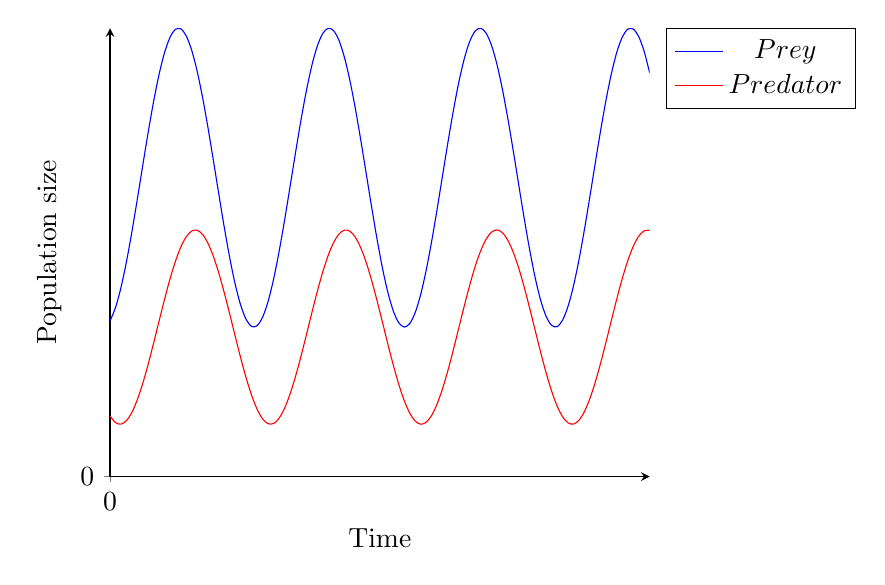
\begin{tikzpicture}
  \begin{axis}[xlabel=Time, ylabel=Population size, xtick={0}, ytick={0}, axis x line=bottom, axis y line =  left, ymin=0, legend pos=outer north east ]
    \addplot[domain=0:15, samples=100, smooth, blue]{2*sin(deg(1.5*x+5))+4};
    \addplot[domain=0:15, samples=100, smooth, red]{1.3*sin(deg(1.5*x+4.3))+2};
    \legend{$Prey$, $Predator$}
  \end{axis}
\end{tikzpicture}
\caption{A graph showing the Lotka-Volterra predator-prey cycle}
\end{center}
\end{figure}



\subsection{\textbf{The SIR Model}}

So far, we have looked at populations alone and with no limiting factors, introduced a carrying capacity due to real world effects and looked at interspecific competition. Now we will look at a model which shows how an infectious disease can progress through susceptible populations to show the likely outcome of an epidemic. This population model is the SIR model which was created in 1927 by W. O. Kermack and A. G. McKendrick. This is a simple model used for modelling epidemics with a fixed population using three variables:

\begin{itemize}
\item $S(t)$ is used to show the number of susceptible individuals at time $t$

\item $I(t)$ is used to show the number of infected individuals at time $t$. These individuals are also capable of spreading the disease via infecting individuals in the susceptible category.

\item $R(t)$ is used to show the number of individuals who have been removed from the disease either by recovering from the disease and becoming immune to reinfection, or by dying as a result of the disease. In this category, individuals cannot spread the disease. [7]
\end{itemize}

The total population is 

$$N=S+I+R.$$[11]

The equations we use for the SIR model are [11 equations 1.5.1, 1.5.2, 1.5.3]:
\begin{align*}
\frac{dS}{dt}&=-\beta SI. \\
\frac{dI}{dt}&=\beta SI - \gamma I. \\
\frac{dR}{dt}&=\gamma I.
\end{align*}

$\beta$ is the transmissivity and this controls the rate at which contacts between $S$ and $I$ hosts cause infection and $\gamma$ is the recovery rate. Because this model is used for populations of a fixed quantity, we can note that $\frac{dN}{dt}=\frac{dS}{dt}+\frac{dI}{dt}+\frac{dR}{dt}=0$ so we can eliminate the variable $R=N-(S+I)$ and ignore the $\frac{dR}{dt}$ equation.


We can find constant solutions to these differential equations, which are called equilibrium points. If we have a differential equation $\frac{dy}{dx} = f(x,y)$, we can find the equilibrium points by setting $\frac{dy}{dx}=0$ and solving for the relevant variable. Once we have found these points, we can determine the nature of each equilibrium to see whether the point is stable, unstable, a saddle point or hyperbolic. To classify each of the equilibrium points, we need to evaluate the jacobian matrix at each one of the points, find the resulting eigenvalues and each equilibrium point can then be determined by finding the eigenvectors associated with the relevant eigenvalue.
 
Once we have found the eigenvalues and eigenvectors of each of the equilibria, we can now classify each of the points. An equilibrium point is stable if all eigenvalues are negative and real, it is unstable if one or both eigenvalues have a positive real part. If one eigenvalue has a positive real part and the other a negative real part, it is a saddle point and if the two eigenvalues have no real parts, it is a hyperbolic fixed point. These equilibrium points can be very useful to find and then classify, so we can understand how the system behaves at these points. For example, at a stable equilibrium point, we know that the system will always return to the point after small disturbances and the system will always move away from the equilibrium point after disturbances when it is unstable.

Having introduced a model that can be used for modeling epidemics and diseases, we can now use this to look at how a disease may affect the red squirrel population. As mentioned before, the rate at which the red squirrel population had been declining was far too steep to be due to habitat or competition alone, so by introducing a model that can model epidemics and diseases, we can look at how a virus (the squirrel pox virus) being introduced to the red squirrels can dramatically affect their population numbers.

\subsection{\textbf{Squirrel Pox}}

Squirrelpox virus is a virus that causes the fatal disease squirrelpox in red squirrels in the UK. The virus is often carried by grey squirrels which were brought into red squirrel habitats from North America. The grey squirrel very rarely dies from squirrel pox since their species has been exposed to the virus for many years so almost all of them have developed immunity. However, they are still carriers of the disease and can transmit it to red squirrels. Unfortunately for the red squirrel species, the squirrel pox is deadly and there are no known red squirrels that have developed immunity. Most die within 15 days of infection [10]. The decline of red squirrels is blamed mostly on disease, loss of woodland habitat and competition with grey squirrels. Seeing the damage of an epidemic like squirrel pox within an environment with red squirrels can be modelled by the SIR model. 




\section{Time to Extinction}

Now, we will look at some factors that will affect the time it takes for a species to become extinct. By looking at these factors, we can assess which ones will affect the declining population of red squirrels in the UK, and use these in our model we will construct to see which one has the biggest impact on them.
 
There are many factors that will affect species’ time to extinction, one being mortality rate outweighing natality rate. As we mentioned in the biological background, the competition for resources between red and grey squirrels has led to red squirrels only having one litter per year and fewer young per litter, so if their mortality rate outweighs this, the red squirrels' time to extinction could dramatically shorten. This also means that an introduction of another competitor is also a factor affecting a species’ time to extinction, as ultimately, it would lead to less red squirrels being able to reproduce.

An unequal offspring sex ratio resulting in either more males than females, or vise versa, would also lead to a declined reproduction rate within the red squirrel population. A destruction of habitat would also massively affect the reproduction rate as we already have evidence of this from the biological background section, whenever woodland habitat was destroyed, red squirrel numbers would decline.

However, as previously mentioned, all of these factors can change over time. Woodland can be destroyed, but also replanted, meaning the numbers can both increase and decrease. So, the factor that we will now look at in our model, is the introduction of a new disease which in this case, will be squirrel pox (a disease that is fatal to red squirrels) that has been carried over by the grey squirrel. An introduction of disease is a factor that could arguably speed up the time to extinction the most out of all the factors we have mentioned, which is why we will investigate it further in our final model using python.

\section{Our Final Model}

Now we will introduce our final complete model, using the following differential equations, representing the SIR populations for both species (note the absence of a recovered red squirrel population, due to inevitable virus fatality):

\begin{enumerate}[label={(\arabic*)}]

\item $\frac{dS_{G}}{dt}=[a_{G}-q_{G}(H_{G}+c_{R}H_{R})]H_{G}-bS_{G}-\beta S_{G}(I_{G}-I_{R})$

\item $\frac{dI_{G}}{dt}=\beta S_{G}(I_{G}+I_{R})-bI_{G}-\gamma I_{G}$

\item $\frac{dR_{G}}{dt}=\gamma I_{G}-bR_{G}$

\item $\frac{dS_{R}}{dt}=[a_{R}-q_{R}(H_{R}+c_{G}H_{G})]H_{R}-bS_{R}-\beta S_{R}(I_{R}+I_{G})$

\item $\frac{dI_{R}}{dt}=\beta S_{R}(I_{G}+I_{R})-(\alpha + b)I_{R}$

\end{enumerate}

With these equations we introduce a number of new parameters relating to different factors in time to squirrel extinction and the introduction of the virus. 

Definition: Parameters with baseline values:

\begin{itemize}
\item $H$=[2,60]  is the proportion of grey to red squirrels initially
\item $I_{G}0$=2 is the number of infected grey squirrels initially
\item $n$=15 the length of study (in years)
\item $b$=0.4 the natural mortality rate of the squirrels
\item $a_{R}$=1 the reproduction coefficient of the squirrels
\item $\alpha=26$ is the virus mortality rate for red squirrels within the simple square
\item $\sigma_{R}=0.61$ is the red competition rate with both species of squirrel
\item $a_{G}$=1.2 is the grey reproduction rate.
\item $\gamma = 13$ is the recovery rate.
\item $\sigma_{G}$=1.65 is the grey competition rate with both species of squirrel.
\end{itemize}

Using these parameters and equations, we can now start modelling how squirrel populations may behave over time for a number of different scenarios. 

\subsection{\textbf{Simple Square Model}}

Our simple square model is a square block of $5km^{2}$ of woodland where we investigate the squirrel populations over time for each of the categories; 

\begin{itemize}
\item Infected red squirrels $I_{R}$
\item Susceptible red squirrels $S_{R}$
\item Infected grey squirrels$I_{G}$
\item Susceptible grey squirrels$S_{G}$
\item Recovered grey squirrels$R_{G}$
\end{itemize}

Within this woodland resides a population of susceptible red squirrels at carrying capacity, so we can assess the impact grey squirrels can have on this population when introduced (with or without the virus) by tracking the numbers in each of these categories over time.

Firstly, if we consider a model containing disease, 2 infected grey squirrels will establish a population and remove the entire red squirrel population (exclusion) after around 12 years, as seen in Figure 4. It is worth understanding here, that without grey squirrels, the infection rate would be completely 0. Without disease, introducing only 2 grey squirrels would not be enough to establish a grey population, possibly due to the competition from the red squirrel population already present - operating at carrying capacity. 

If we consider a model without the virus, competition alone would not be sufficient to achieve red exclusion if only 2 grey squirrels were introduced at the beginning. You would actually need at least 18 grey squirrels to be introduced into the population to achieve red squirrel exclusion and with competition alone the time to extinction is around 40 years - over three times as long.

This clearly demonstrates the impact the parapox virus has on the red squirrel population. In Figure 8 we can see that the immediate infection and decline of the initial population from carrying capacity aids the greys in establishing their own population at a significantly increased rate. This is likely due to the reduction of crowding and competition from this initial decline - wherein the grey squirrel population benefits from more so - on account of their greater reproductive and growth rates [1]. This is again compounded by the fact that red squirrels are less efficient with food resources than their grey counterparts, contributing to a greater susceptibility to competitive effect and eventual exclusion [1]. In summary, not only is the time to red squirrel exclusion greatly reduced in the presence of the virus, but the initial number of grey squirrels required for red squirrel exclusion is significantly less also.


\begin{figure}[H]
\begin{center}
\includegraphics[width=0.7\textwidth]{sirgraph}
\caption{The two squirrel populations, showing the dynamics of population numbers after the introduction of two infected grey squirrels.}
\end{center}
\end{figure}

\begin{figure}[H]
\begin{center}
\includegraphics[width=0.7\textwidth]{population}
\caption{A comparison of the two squirrel populations with and without the presence of disease, showcasing the acceleration of red squirrel exclusion when disease is present.}
\end{center}
\end{figure}

\subsection{\textbf{Results for Changing Parameters}}

If we change the virus transmission coefficient $\beta$, the virus mortality rate $\alpha$, the proportion of red squirrels to grey squirrels, changing the reproduction rate of red and grey squirrels, we want to see how they affect extinction or exclusion. To compare this we will be using the baseline coefficients we introduced at the start of the model (refer back to Parameters Definition in Section $6$ to see the baseline).

Firstly, we investigated the effect of the virus transmission coefficient on the time to red squirrel exclusion. As seen in Figure $10$, a reduction in $\beta$ by as little as $0.1$ leads to an increase in the time taken for exclusion to occur by $6$ years, and a further reduction of only $0.05$ results in almost twice the number of red squirrels still alive after $11$ years. In order for the infection to completely die out, the virus transmission coefficient must be reduced to as low as $0.52$, where competition remains the only factor in play. The $25\%$ decrease of transmission efficiency still prompts the same conclusion, it is testament to the serious impact the parapox virus has on red squirrels even at a reduced potency.
 
\begin{figure}[H]
\begin{center}
\includegraphics[width=0.7\textwidth]{diseasetransmission}
\caption{Exhibiting how incremental decrease in disease transmission efficiency can increase time to extinction.}
\end{center}
\end{figure}

Secondly, if you increase the red squirrel virus mortality rate, $\alpha$ from 26 per year to 35 per year this still culminates in their exclusion, demonstrated in Figure 11, as does any reduction in this number, for instance the reduction to 19 per year as seen in Figure 11. At the higher end of this spectrum, the squirrels are dying at a much faster rate - reducing the time spent infected and thus infecting fewer squirrels. This increase of over 25\% still results in red squirrel decline and complete exclusion. Conversely, a reduction in the mortality rate leads to a greater number of new squirrels infected per carrier, due to more squirrels surviving the virus, increasing the number of carriers of the virus in the population. Hence this decreases the time needed to infect the entire red squirrel population as the number infected at each time point is greater. It is this effect that has the greatest power in reducing time to exclusion, as seen in Figure 11.

\begin{figure}[H]
\begin{center}
\includegraphics[width=0.7\textwidth]{mortality}
\caption{A comparison of the two squirrel populations under varying rates of red squirrel virus mortality. }
\end{center}
\end{figure}

Next we want to investigate how the initial proportion of red squirrels to grey squirrels affects the time to extinction. Here we are keeping the number of infected grey squirrels the same but we changed the number of susceptible grey squirrels introduced into the system. As seen in Figure 12, an increase of one grey squirrel decreases the time to extinction by roughly 15\%, and the time to extinction is 2 years sooner. As before with other coefficients, we might have wanted to show the trend with a reduction by one grey squirrel, however with a reduction we have to change the number of infected grey squirrels initially added. This is not a suitable comparison because we have changed the number infected which would have an impact. This is because we cannot tell from this where the impact for less initially infected squirrels and what the effect of lowering the proportion to [1,60] had. 

\begin{figure}[H]
\begin{center}
\includegraphics[width=0.7\textwidth]{addinggrey}
\caption{Showing the impact adding an additional single, uninfected grey squirrel has on time to extinction in comparison baseline.}
\end{center}
\end{figure}

If we change the reproductive coefficient for both ($a_{R}$ and $a_{G}$), firstly testing if we decrease $a_{G}$ by 0.2 and increasing $a_{R}$ by 0.2, and then the converse. Here it is necessary to note that to allow for crowding, we have additional factors of population density based on the reproduction rate and the natural mortality rate divided by carrying capacity, denoted as $k_{R}$, which we defined in this example to be 60. We added this factor because the crowding would have an effect on the number of additional members of the population due to resources such as availability of breeding grounds and nesting areas, as well as food availability. All of these are less available with a greater population. For the first test, using an increase in $a_{R}$ and a decrease in $a_{G}$, we found that extinction occurred around 15 years and for the latter test extinction was approximately 9 years, as seen in Figure 13. This shows an increase in 25\% if we increase the $a_{R}$ and decrease the $a_{G}$, and if we increase $a_{G}$ and decrease $a_{R}$ decreases the time to extinction by 25\%. 

\begin{figure}[H]
\begin{center}
\includegraphics[width=0.7\textwidth]{reproductiverates}
\caption{A comparison of how varying the reproductive rates impacts the time to extinction.}
\end{center}
\end{figure}

It is also useful to note that even when allowing minor fluctuations in parameter values such as these, there is no doubt that the extinction of red squirrels is greatly accelerated in the presence of the squirrelpox virus. This in itself reflects the impact the virus can have on squirrel populations, but also implies that even with slight variations or small errors the conclusion here remains the same. Broadly speaking, this is testament to both the robustness of our results, and also the stark contrast in time to extinction versus competition alone.

Realistically, we can implement most of these parameter changes by changing the environment. For example an expansion of woodland at the beginning of the introduction of grey squirrels in the early 1900s would likely have delayed the predicted extinction for within the next decade. The issue with expanding the woodland areas is the length of time needed for these trees to grow to suitable heights for squirrels to live in is too long to implement now to slow down or stop the extinction of red squirrels. If more trees had been planted 40 years earlier, then we would likely be seeing many more red squirrels, as this increase in habitat would trigger an increase in the reproductive rate for both species. Furthermore, this would have the potential to decrease the initial infection rate, due to the squirrels having a larger habitat, so the dreys are likely to be more spread out across more trees - resulting in less contact between squirrels - hence a reduced spread of disease. Of course this is only a temporary solution, as once the numbers of squirrels grow to a stage where population density increases, then the virus transmission would eventually increase to a similar stage to what it is now. 

Equally, another strategy for implementing these parameter changes would be to implement red squirrel only forests as mentioned in Professor White’s lecture [9]. This would eliminate the virus altogether as with no grey squirrels carriers, then no red squirrels can get infected with the virus. This is an effective plan however the forests would likely be surrounded by other woodland areas, which would have grey squirrels living in. This creates an issue because if there are places where red and grey squirrels can get close enough together on opposite sides of a fence they can still spread the virus between them. Not only this but squirrels can probably climb most if not all fences. 


\section{An Extension}

As an extension, we investigated the role disease plays in the exclusion of red squirrels, in conjunction with migration. This was achieved using a small, square grid full of red squirrels and releasing one breeding pair of grey squirrels into a single population/square. This simulates the introduction of grey squirrels to the UK ,as seen in the late 1800’s and early 1900’s [9]. The squirrels in each square can then migrate to neighbouring squares in the grid after each year that passes, possibly introducing the virus into a new squirrel population. These populations can be tracked over time to more accurately assess the interactions between migration, disease and competition within a larger ecosystem.

This idea was presented in a lecture we watched [9] and is also explored in “Ecological replacement of native red squirrels by invasive greys driven by disease,” [1]. The idea was to investigate the spread of grey squirrels against the depletion of the red squirrel population in the highlands of Scotland in order to predict the state of the squirrel population in the future. We thought that this idea was interesting, and so wanted to investigate ourselves. Firstly we wanted to get an idea of the study, so we coded for the spread of disease through a simple square model.

Our original idea was to split a large area into smaller tiles which would create a grid concept. From this, we thought an interesting concept would be to measure how limiting movement would affect the spread of the virus. 

\subsection{\textbf{Simple Square Model}}

To start our extension, we investigated the simple square model we made earlier. As before, it represents a tile of $5km^{2}$ of woodland habitat. Our goal was to represent the migration of disease around the tile. In this version, we had a population of 60 red squirrels and 2 grey squirrels in a tile and from this we found the yearly depletion in the red squirrel population. This means that the simple model does not demonstrate a model in which the grey squirrels are added and the infection has to migrate its way through the population. Not only this, our model only showed the infection spreading through a small contained space and so we wondered what would happen if we had a collection of these tiles. From this we developed our next idea for a grid model system.

\subsection{\textbf{Grid Model}}

We set up a 11 by 11 unit grid in python, with each tile representing a $5km^{2}$ patch of woodland - containing values for the number of susceptible, infected and recovered grey squirrels, and susceptible and infected red squirrels within the square. After each year, we found the population of this grid, and in conjunction with the results from the simple square model, a comparison can be made of how the grid model affects the accuracy population size found at each time point. The difference between these two models is that the simple model covers only one $5km^{2}$ area of woodland, but in the grid model squirrels are able to migrate away from their original square to adjacent tiles making this a more realistic interpretation of the system. 

Firstly, we placed 60 red squirrels (carrying capacity) in all the tiles and the two grey squirrels into one of the tiles, simulating the introduction in the early 1900s. The total number of squirrels migrating away from a square is calculated using a dispersion factor, denoted as ${\mu}$. The dispersion factor is the expected portion of the population in one tile to migrate out of the tile, so using this we  find an extrapolation of the population movement from one tile to a single one of  one of the neighbouring tiles by using: 

$$\textrm{(population in tile)} \times \mu \times \frac{1}{8}$$

As there are 8 neighbouring tiles normally, the possible migration pattern for a squirrel in a start tile is depicted in the picture below:

\begin{figure}[H]
\begin{center}
\includegraphics[width=0.5\textwidth]{3x3}
\caption{A diagram of possible migration patterns in the grid model.}
\end{center}
\end{figure}

In Figure 14, we can assume that the migration is evenly spread through all of the possible tiles, so the migrating population multiplied by $\frac{1}{8}$ gives the total population to move from one tile to a single one of the neighbouring tiles. 

One problem that we faced was if a tile was at the edge of the grid, then the migrating squirrel population had nowhere to go in a certain direction. We found that a solution was to prevent migration from happening in this direction. So, in this grid there are 40 tiles which fit this category, so the migrating population in the direction of leaving the grid would not be allowed to leave, instead remaining in the tile from whence it came. This allows for consistent movement as with the other unrestricted tiles. In a realistic context, this creates a portion of woodland which is either enclosed by a fence stopping the squirrels from escaping, or surrounded by an unsuitable habitat for squirrels to thrive.

\subsection{\textbf{Result}}

The output of these models shows that the simple square model exhibits red squirrel extinction much earlier. If we define extinction to occur when the population output is less than 1, then the simple square model shows signs of extinction at around 12 years. In contrast, the grid model shows signs of exclusion much later around 65 years as seen in Figure 15. This contrast is likely due to the time needed for the grey squirrels to travel into other tiles within the grid from the starting tile, and so only the squirrels from within in the grey squirrel starting tile are vulnerable to the virus at the beginning. Conversely, all of the squirrels in the simple square model are vulnerable to the disease from the start. This idea for the grid model is more accurate to reality as it is likely that grey squirrels would find a habitat and remain close to that habitat especially during the each of the bi-yearly breeding season. This informs us that the squirrel population infected by one grey squirrel would be likely to be within a reasonably small radius around the drey (the grey squirrel’s nest) [3] of that grey squirrel. 

\begin{figure}[H]
\begin{center}
\includegraphics[width=0.9\textwidth]{exclusion}
\caption{Graph to show the time to exclusion of the grid model versus the simple square model.}
\end{center}
\end{figure}

In a realistic context, it would be unlikely that squirrels could be contained within a fence because they are tree dwellers so would likely be able to climb out of an enclosed environment. One containment method could be to have an electric fence but realistically that would likely affect the movement of the squirrels as they might avoid the fence. Equally, another option could be to enclose the area using a fence with netting overhead as well. This would likely be a more effective containment method as the model would likely be unchanged and migration still randomized. Another containment method could be geographical limitations such as the grid of woodland surrounded by water or by habitat unlike a squirrels habitat, such as urban areas or fields.  In these environments the squirrels will not migrate out of the ideal squirrels habitat to these unideal habitats and conditions. In spaces where the habitat is surrounded by urban areas however you might see a similar outcome as the introduction of the electric fence.This is because the urban area is likely to have a lot of traffic which could cause the squirrels to be less likely to migrate towards the edges of the habitat. 

One way to further our investigation here is to create a break function, where we define that if the population of susceptible red squirrels falls below a point then the circuit breaks and we get an output of the number of years until extinction for both. In this, we need to define a suitable point where extinction occurs, and for this we had two ideas; either extinction when the population density of susceptible red squirrels ($S_{R}$) is less than 1 or when $S_{R}$ is less than 2. We chose to investigate the susceptible population as this virus is lethal to all red squirrels so we can assume that if a red squirrel is infected, that it will not be alive by the next time point. We also consider extinction to happen at a time point where the population cannot recover and begin to increase, so reproduction cannot occur. 

Firstly, if the extinction point is less than 1, then this identifies in our study that there are no ‘whole squirrels’ left in the population which defines extinction. It is important to note here that the population realistically would not necessarily be 60 in this square however we have decided to consider the population density here as the population. From this we can conclude that the reproductive rate drops to zero as the requirement for reproduction is at least 2 squirrels in the population. Even if the virus and competition factors were to be removed here, the squirrel density means that there cannot be any increase in population so once this one squirrel died of natural causes, then we know the red squirrels are extinct. 

Alternatively, if we were to set when SR is less than 2 as the extinction point, then the population would consist of less than 2 squirrels in our model. This would lead to extinction because of the need for 2 healthy red squirrels in the population in order for the reproduction rate to not drop to zero so with less than 2, the reproduction rate is 0 and so there can be no recovery for the population in this closed grid, leading to a density of no squirrels remaining. 



\section{Conclusion}

Through our discussion of factors affecting red squirrel population decline, we have established that although other factors such as habitat and competition have affected the declining red squirrel population, none of them have affected them as much as the squirrelpox virus. We have modelled how the red and grey squirrel population could change overtime if it was purely based on competition, finding that it would take 18 uninfected grey squirrels around 40 years to wipe out the red squirrel population. Whereas looking at a model with disease, it would take 2 infected grey squirrels around 12 years to wipe out the red squirrel population. This again reinforces the idea that squirrelpox has played a massive role in the steep decline of the number of red squirrels over the past few years, and that the conservation efforts being made by the government to protect the remaining population is completely justified.




\section{Works Cited}

\begin{enumerate}[label={[\arabic*]}]

%1
\item D. Tompkins, A. White and M. Boots, \emph{Ecological Replacement of Native Red Squirrels by the invasive Grey driven by Disease}, University of Sterling, University of Heriot Watt, 2003. [Online]. Available: \url{http://www.macs.hw.ac.uk/~awhite/Tompkins_etal_EL2003.pdf}.
%2
\item Unknown, \emph{Scottish Red Squirrels}, [Online]. Available: \url{https://scottishsquirrels.org.uk/2019/02/21/how-many-red-squirrels-are-there-in-scotland/#:~:text=Do\%20we\%20know\%20how\%20many\%20red\%20squirrels\%20there\%20are\%20in\%20Scotland\%3F&text=It's\%20been\%20estimated\%20that\%20there,very\%20much\%20a\%20ballpark\%20figur}. [Accessed 1 december 2020].
%3
\item RSPB, /emph{Birds and Wildlife}, [Online]. Available: \url{https://www.rspb.org.uk/birds-and-wildlife/wildlife-guides/other-garden-wildlife/mammals/grey-squirrel/#:~:text=Their\%20nest\%2C\%20called\%20a\%20drey,\%2C\%20leaves\%2C\%20bark\%20and\%20grass}. [Accessed 30 november 2020].
%4
\item Khan Academy, \emph{Population ecology - Logistics Graph}, [Online]. Available: \url{https://www.khanacademy.org/science/ap-biology/ecology-ap/population-ecology-ap/a/exponential-logistic-growth}. [Accessed 2 december 2020].
%5
\item Wikipedia, \emph{Volterra Equations}, [Online]. Available: \url{https://en.wikipedia.org/wiki/Lotka\%E2\%80\%93Volterra_equations}. [Accessed 20 November 2020].
%6
\item J. Olsen, \emph{Modelling Interspecific Competition}, 8 October 2014. [Online]. Available: \url{https://www.youtube.com/watch?v=obasfCufOr0}. [Accessed 20 November 2020].
%7
\item Wikipedia, \emph{Modelling of Infectious Disease}, Wikipedia, [Online]. Available: \url{https://en.wikipedia.org/wiki/Mathematical_modelling_of_infectious_disease}. [Accessed 5 November 2020].
%8
\item T. W. Trust, \emph{Red squirrel conservation}, [Online]. Available: \url{https://www.lancswt.org.uk/our-work/projects/red-squirrel-conservation}. [Accessed 15 November].
%9
\item A. White, \emph{Prof. Andy White: Red Squirrel Conservation in a Mathematical Nutshell}, 3 November 2014. [Online]. Available: \url{https://www.youtube.com/watch?v=WVk6ubTNEoc}. [Accessed 25 November 2020].
%10
\item N. Squirrels, \emph{Northern Red Squirrels}, [Online]. Available: \url{http://www.northernredsquirrels.org.uk/squirrels/squirrel-pox-virus/}. [Accessed 25 November 2020].
%11
\item A. Best and N. Monk, Logistic equation, Interacting populations: Competition, Modelling epidemics in human populations,” in \emph{Logistic modelling, Exponential model, Modelling epidemics in human populations}, Sheffield, University of Sheffield, 2020, pp. 4, 12:15, 22.
%12
\item Wikipedia, \emph{Squirrelpox Virus}, [Online]. Available: \url{https://en.wikipedia.org/wiki/Squirrelpox_virus}. [Accessed 25 November 2020].
%13
\item \emph{Figure of Population Depletion}, [Online]. Avaliable: \url{https://www.wildlifetrusts.org/saving-species/red-squirrels}. Accessed 10 December 2020] 
%14
\item \emph{Diagram Size Comparison}, [Online]. Available: \url{https://gardeningwithchildrenblog.co.uk/tag/red-squirrel-conservation/}. [Accessed 20 November 2020].

\end{enumerate}




\section{Bibliography}

\begin{verbatim}

# -*- coding: utf-8 -*-
"""
Created on Sun Nov 29 16:35:19 2020

@author: Zach
"""
import numpy as np
import matplotlib.pyplot as plt
from scipy.integrate import odeint 

b = 0.4 # Natural mortality rate (per year)
beta = 0.7 # Virus transmission rate
mew = 0.2 # Dispersal fraction to neighbouring tiles (After 1 year)
n = 80 # Number of years
t = np.linspace(0, n, 200) # A grid of time points (in days)

aR = 1.0 # Reds max reproductive rate
KR = 60 # Reds carrying capacity
alpha = 26 # Reds virus mortality rate
sigmaR = 0.61 # Reds competition effect (on Greys)
qR = (aR - b)/KR # Reds rate of susceptibility to crowding

aG = 1.2 # Greys max reproductive rate
KG = 80 # Greys carrying capacity
gamma = 13 # Virus recovery rate
sigmaG = 1.65 # Greys competition effect (on Reds)
qG = (aG - b)/KG # Greys rate of susceptibility to crowding


H = [2,60] # Total population [Grey,Red]
HG, HR = H
RG0 = 0 # Recovered Greys initially 0

IG0 = 2 # Infected Greys initially
SG0 = HG - IG0 - RG0 # Susceptible Greys 

IR0 = 0 # Infected Reds initially 0
SR0 = HR - IR0 # Susceptible Reds 


# The L-V/SIR model differential equations.
def deriv(y, t):
    SG, IG, RG, SR, IR = y
    HG = SG + IG + RG
    HR = SR + IR
    dSGdt = (aG-qG*(HG+sigmaG*HR))*HG - b*SG - beta*SG*(IG+IR)
    dIGdt = beta*SG*(IG+IR)-b*IG-gamma*IG
    dRGdt = gamma*IG - b*RG
    dSRdt = (aR-qR*(HR+sigmaG*HG))*HR - b*SR - beta*SR*(IR+IG)
    dIRdt = beta*SR*(IG+IR) - (alpha+b)*IR 
    return dSGdt, dIGdt, dRGdt, dSRdt, dIRdt

# Initial conditions vector
y0 = SG0, IG0, RG0, SR0, IR0
ret = odeint(deriv, y0, t)
SG, IG, RG, SR, IR = ret.T

grey_total = SG + IG + RG
red_total = SR + IR



'''Grid Model'''

rdim = 10 # 11 rows
cdim = 10

yt = odeint(deriv, (0, 0, 0, 60, 0), [t[0]]).flatten()
 # Creates a yt for each timestamp

yt_grid = np.zeros(((rdim+1),(cdim+1),5))
for i in range(rdim+1):
    for j in range(cdim+1):
        yt_grid[i,j] = yt

yt_grid[0,0] = np.array([0, 2, 0, 60, 0])

SG1, SR1 = [2], [60*121]

for i in range(1,len(t)):        # len(t)
    if np.floor(t[i]) - np.floor(t[i-1]) == 1: # Checks if end of yr
        yt_prop = yt_grid * mew * 0.125
        yt_changeover = np.zeros(((rdim+1),(cdim+1),5))
        print('Year:', int(t[i]))
        for r in range(rdim+1):
            for c in range(cdim+1):
                if r == c == 0:
                    #print("Top Left Corner")
                    yt_changeover[r,c] += - yt_prop[r,c]*3
                    yt_changeover[r,c+1] += yt_prop[r,c]
                    yt_changeover[r+1,c+1] += yt_prop[r,c]
                    yt_changeover[r+1,c] += yt_prop[r,c] 
                elif r==0 and c==rdim:
                    #print("Top Right Corner")
                    yt_changeover[r,c] += - yt_prop[r,c]*3
                    yt_changeover[r,c-1] += yt_prop[r,c]
                    yt_changeover[r+1,c-1] += yt_prop[r,c]
                    yt_changeover[r+1,c] += yt_prop[r,c]                 
                elif r==cdim and c==0:
                    #print("Bottom Left Corner")
                    yt_changeover[r,c] += - yt_prop[r,c]*3
                    yt_changeover[r,c+1] += yt_prop[r,c]
                    yt_changeover[r-1,c+1] += yt_prop[r,c]
                    yt_changeover[r-1,c] += yt_prop[r,c]                  
                elif r == c == rdim:
                    #print("Bottom Right Corner")
                    yt_changeover[r,c] += - yt_prop[r,c]*3
                    yt_changeover[r,c-1] += yt_prop[r,c]
                    yt_changeover[r-1,c-1] += yt_prop[r,c]
                    yt_changeover[r-1,c] += yt_prop[r,c]                    
                elif r == 0:
                    #print("Top Row")
                    yt_changeover[r,c] += -yt_prop[r,c]*5
                    yt_changeover[r,c+1] += yt_prop[r,c]
                    yt_changeover[r+1,c+1] += yt_prop[r,c]
                    yt_changeover[r+1,c] += yt_prop[r,c]
                    yt_changeover[r+1,c-1] += yt_prop[r,c]
                    yt_changeover[r,c-1] += yt_prop[r,c]
                elif c == 0:
                    #print("Left Column")
                    yt_changeover[r,c] += -yt_prop[r,c]*5
                    yt_changeover[r-1,c] += yt_prop[r,c]
                    yt_changeover[r-1,c+1] += yt_prop[r,c]
                    yt_changeover[r,c+1] += yt_prop[r,c]
                    yt_changeover[r+1,c+1] += yt_prop[r,c]
                    yt_changeover[r+1,c] += yt_prop[r,c]                    
                elif r == rdim:
                    #print("Bottom row")
                    yt_changeover[r,c] += -yt_prop[r,c]*5
                    yt_changeover[r,c-1] += yt_prop[r,c]
                    yt_changeover[r-1,c-1] += yt_prop[r,c]
                    yt_changeover[r-1,c] += yt_prop[r,c]
                    yt_changeover[r-1,c+1] += yt_prop[r,c]
                    yt_changeover[r,c+1] += yt_prop[r,c]                    
                elif c == cdim:
                    #print("Right Column")
                    yt_changeover[r,c] += -yt_prop[r,c]*5
                    yt_changeover[r-1,c] += yt_prop[r,c]
                    yt_changeover[r-1,c-1] += yt_prop[r,c]
                    yt_changeover[r,c-1] += yt_prop[r,c]
                    yt_changeover[r+1,c-1] += yt_prop[r,c]
                    yt_changeover[r+1,c] += yt_prop[r,c]                    
                else:
                    #print("Central Squares")
                    yt_changeover[r,c] += -yt_prop[r,c]*8
                    yt_changeover[r-1,c] += yt_prop[r,c]
                    yt_changeover[r-1,c+1] += yt_prop[r,c]
                    yt_changeover[r,c+1] += yt_prop[r,c]
                    yt_changeover[r+1,c+1] += yt_prop[r,c]
                    yt_changeover[r+1,c] += yt_prop[r,c]
                    yt_changeover[r+1,c-1] += yt_prop[r,c]
                    yt_changeover[r,c-1] += yt_prop[r,c]
                    yt_changeover[r-1,c-1] += yt_prop[r,c]
                    
        yt_grid += yt_changeover
        
    for p in range(rdim+1):
        for q in range(cdim+1):
            yt_grid[p,q] = odeint(deriv, yt_grid[p,q].flatten(), [t[i-1], t[i]])[1]
    # print(yt_grid[0,0,3], ret[i,3])
    # Output here compares S reds.
    # Left output is grid model, right is single square
    SG1 = np.append(SG1, [sum(sum(yt_grid[0:,0:,0]) + 
	                              sum(yt_grid[0:,0:,1]) + sum(yt_grid[0:,0:,2]))])
    SR1 =  np.append(SR1, [sum(sum(yt_grid[0:,0:,3]) + 
	                               sum(yt_grid[0:,0:,4]))])






fig, ax = plt.subplots(ncols=2,sharey=True)
ax[1].plot(t, SG1/121, 'black', alpha=0.7, lw=2, label='Grey Population')
ax[1].plot(t, SR1/121, 'red', alpha=0.8, lw=2, label='Red Population')
ax[0].plot(t, grey_total, 'black', alpha=0.7, lw=2, label='Grey Population')
ax[0].plot(t, red_total, 'red', alpha=0.8, lw=2, label='Red Population')
ax[0].set_box_aspect(1)
ax[1].set_box_aspect(1)
ax[0].set_xlabel('Time (years)')
ax[1].set_xlabel('Time (years)')
ax[0].set_ylabel('Population')
ax[0].set_title('Simple Square Model')
ax[1].set_title('Grid Model')
fig.suptitle('Graphs comparing the time to red squirrel exclusion \n 
	in the two models.', fontsize=16)
fig.tight_layout()
legend1 = ax[1].legend(loc='upper left', fontsize=9)
legend1.get_frame().set_alpha(0.5)
legend0 = ax[0].legend(loc='right', fontsize=9)
legend0.get_frame().set_alpha(0.5)
plt.show()



\end{verbatim}








\end{document}